\documentclass[11pt]{article}
\usepackage[margin=1in]{geometry}
\usepackage{amsmath,amssymb,amsthm,mathtools}
\usepackage{graphicx}
\usepackage{booktabs}
\usepackage{enumitem}
\usepackage{tikz}
\usetikzlibrary{positioning,arrows.meta}
\usepackage[colorlinks=true,linkcolor=blue,citecolor=blue,urlcolor=blue]{hyperref}

\newtheorem{theorem}{Theorem}
\newtheorem{corollary}[theorem]{Corollary}
\newtheorem{lemma}[theorem]{Lemma}
\newtheorem{proposition}[theorem]{Proposition}
\theoremstyle{definition}
\newtheorem{definition}[theorem]{Definition}
\newtheorem{remark}[theorem]{Remark}
\newtheorem{conjecture}[theorem]{Conjecture}

\newcommand{\N}{\mathbb{N}}
\newcommand{\cP}{\mathcal{P}}
\newcommand{\NOR}{\operatorname{NOR}}
\newcommand{\low}{\operatorname{low}}

\title{Subtraction Games Can Count:\\ Exponentially Long Periods and a Counterexample to Guy's Conjecture}
\author{}
\date{September 2026}

\begin{document}
\maketitle

\begin{abstract}
In the subtraction game with a finite move set $S\subset\N_{>0}$, a heap of $n$ tokens is reduced
by some $s\in S$ per move and the player who cannot move loses.  The sequence of winning/losing
positions is eventually periodic, and a long-standing question, going back to R.~K.~Guy, asks how
long the period can be.  Guy conjectured that the period is bounded by a polynomial of degree
$\binom{n}{2}$ in the largest move when $|S|=n$; Flammenkamp (1997) observed experimentally that
the period of some five-move games seems to grow exponentially, and whether exponential periods
are possible at all has remained open (Miklós--Post 2024, Larsson--Saha 2024).

We settle the question.  We construct an explicit family of subtraction sets $S_k$ with at most
$54$ moves each and $\max S_k< 377(k+1)$ whose outcome sequence has least period
\emph{exactly} $377\cdot k\cdot 2^{k}$.  Hence periods of subtraction games with a bounded number of
moves are not bounded by any polynomial in the largest move: Guy's conjecture is false, both for
outcome sequences and for nim-sequences, and Flammenkamp's conjecture is true.  The construction
shows that a subtraction game is a \emph{nonlinear feedback shift register whose feedback is a NOR
gate}; by laying out wires, clocks and ``covering'' residues inside blocks of length $B=377$ we make
the game simulate a bit-serial binary counter.  The layout was discovered by computer search
(randomised Sidon-type constructions, greedy set cover and simulated annealing, reducing the
number of moves from $1061$ to $54$), and \emph{every} step of the proof---the general simulation
theorem, the correctness of the counter, the finite layout conditions, the exact least period, and
the failure of Guy's bound---has been formally verified in the Lean~4 proof assistant with
Mathlib, using only the standard axioms.

More generally we prove a \emph{General Layout Lemma}: every synchronous NOR circuit with delay
lines is simulated by a one-heap subtraction game of polynomial size.  As a consequence, deciding
whether a given heap size $n$ (in binary) is a P-position of a given subtraction game (in unary) is
PSPACE-complete, and EXPTIME-complete when the moves are written in binary, whereas for every
\emph{fixed} one-heap game the question is easy.
\end{abstract}

\section{Introduction}

Let $S\subset\N_{>0}$ be finite.  In the \emph{subtraction game} $S$ a position is a heap of
$n\ge 0$ tokens; a move removes $s\in S$ tokens provided $s\le n$; under normal play the player
unable to move loses.  A position is a \emph{P-position} (a win for the Previous player) iff every
move leads to a non-P-position:
\begin{equation}\label{eq:P}
  n\in\cP_S \iff \bigl(n-s\notin \cP_S \text{ for every } s\in S \text{ with } s\le n\bigr).
\end{equation}
Equivalently, $\cP_S$ is the \emph{greedy} subset of $\N$ containing no two elements whose
difference lies in $S$.  Writing $w(n)=1$ if $n\in\cP_S$ and $w(n)=0$ otherwise, \eqref{eq:P} reads
\[ w(n)=\NOR\bigl(w(n-s): s\in S\bigr), \qquad w(\text{negative})=0. \]
Thus $w$ is generated by a shift register of length $m=\max S$ with a NOR feedback function.  By the
pigeonhole principle it is eventually periodic, with period at most $2^m$.

Subtraction games are the first problem in Nowakowski's \emph{Unsolved Problems in Combinatorial
Games}~\cite{Nowakowski}:
\begin{quote}
``In general, period lengths can be surprisingly long, and it has been suggested that they could
be super-polynomial in terms of the size of the subtraction set.  However, Guy conjectures that they
are bounded by polynomials of degree at most $\binom{n}{2}$ in $s_n$, the largest member of a
subtraction set of cardinality $n$.''
\end{quote}
Althöfer and Bültermann~\cite{AB} found families with cubic period and asked whether
super-polynomial periods occur for $|S|\ge 5$.  In his thesis, Flammenkamp~\cite{Flammenkamp}
computed record periods of ``max-symmetric'' five-move sets and observed growth like
$2^{0.3\max S}$; this observation is recorded as Conjecture~1 in the recent survey of Larsson and
Saha~\cite{LS}.  Miklós and Post~\cite{MP} write that ``it is a long time open question if
exponential period length is possible''; they proved super-polynomial periods $e^{\Omega(\sqrt{\max S})}$
for a \emph{modified} game in which the outcomes of the first few positions are prescribed by a
seed.  For the actual game no super-polynomial example was known.

\subsection{Main results}

\begin{theorem}[Exponential periods]\label{thm:main}
There is an explicit family of finite sets $S_k\subset\N_{>0}$ $(k\ge 2)$ such that
\begin{enumerate}[label=(\roman*)]
\item $|S_k|\le 54$ and every $s\in S_k$ satisfies $0<s<377(k+1)$;
\item the outcome sequence of the subtraction game $S_k$ is eventually periodic with least period
exactly $377\cdot k\cdot 2^{k}$.
\end{enumerate}
\end{theorem}

Since the nim-value of a position is $0$ exactly at P-positions, every period of the nim-sequence is
a period of the outcome sequence; hence the least period of the nim-sequence of $S_k$ is a
multiple of $377\,k\,2^k$ as well.

\begin{corollary}[Guy's conjecture fails]\label{cor:guy}
For every $C,d\ge 1$ there is a subtraction set $S$ with at most $54$ moves whose outcome period
(and nim-period) exceeds $C\,(\max S)^d$.  In particular the periods of subtraction games with
$n=54$ moves are not bounded by a polynomial of degree $\binom{54}{2}$ in $\max S$.
\end{corollary}

Concretely, $S_{33750}$ has $54$ moves, largest move $\max S=12\,723\,737$, and period
$377\cdot 33750\cdot 2^{33750}>(\max S)^{\binom{54}{2}}$; $k=33750$ is the smallest $k$ for which
this happens.

\begin{theorem}[see Section~\ref{sec:pspace}]
Given $S$ in unary and $n$ in binary, deciding whether $n$ is a P-position of $S$ is
PSPACE-complete.
\end{theorem}

\paragraph{Related work.}  Larsson and Wästlund~\cite{LW} and Larsson~\cite{L12} showed that
subtraction games on \emph{two or more} heaps emulate one-dimensional cellular automata (a ``time
heap'' and a ``tape heap''), yielding undecidability results; Gurvich and Vyalyi~\cite{GV} proved
PSPACE-hardness and exponential lower bounds for fixed multidimensional games, and subtraction games
played on graphs are PSPACE-complete~\cite{DGPS}.  For one heap, where
the outcome sequence is always eventually periodic, we are not aware of any hardness result.  Our construction
packs space and time into a \emph{single} heap by cutting it into blocks.

\paragraph{Formal verification.}  Theorem~\ref{thm:main}, Corollary~\ref{cor:guy}, the nim-sequence statement
and the General Layout Lemma are proved in Lean~4 with Mathlib (Section~\ref{sec:lean}), with main statements
\begin{itemize}
\item \texttt{SubGame.Concrete.exponential\_period} (Theorem~\ref{thm:main}),
\item \texttt{SubGame.Concrete.guy\_fails} and \texttt{not\_polynomially\_bounded} (Corollary~\ref{cor:guy}),
\item \texttt{SubGame.Concrete.nim\_period\_dvd} (nim-sequences),
\item \texttt{SubGame.GLL.simulate} (General Layout Lemma);
\end{itemize}
{\sloppy The command \texttt{\#print axioms} reports only \texttt{propext}, \texttt{Classical.choice} and \texttt{Quot.sound}.
The PSPACE-completeness theorem is proved on paper; its game-theoretic core is part of the formal
development, while the standard encoding of a linear-bounded automaton as a cellular automaton is not
formalised.\par}

\subsection{Idea of the construction}

The recursion $w(n)=\NOR(w(n-s):s\in S)$ applies the \emph{same} NOR gate at every position.  We
cut $\N$ into blocks of length $B$ and give every residue $r\in\{0,\dots,B-1\}$ a role:
\begin{itemize}
\item \emph{clocks} $r\in C$: $w(\tau B+r)=1$ for all blocks $\tau$;
\item \emph{zero residues}: $w(\tau B+r)=0$, forced by a move landing on a clock;
\item \emph{wires} $r=\rho(j)$: the value $w(\tau B+\rho(j))$ is a logical signal $\ell_j(\tau)$.
\end{itemize}
A move $s=qB+\delta$ applied at a wire at residue $e$ reads residue $(e-\delta)\bmod B$ in an earlier
block.  If the residues are arranged so that each wire ``sees'' exactly its intended inputs and never a
clock, and clocks see nothing but zero residues, then every wire computes a NOR gate of chosen
inputs with chosen delays (Theorem~\ref{thm:sim}).  NOR gates are universal, and a move of length
about $kB$ gives a delay line of $k$ blocks.  We use this to build a bit-serial binary counter
whose $k$-bit word is stored in the delay line: the game counts from $0$ to $2^k-1$ over and over,
and the period is exactly $k\cdot 2^k$ blocks.

\section{The simulation theorem}\label{sec:sim}

\begin{definition}[Design]
A \emph{design} consists of a block length $B\ge 1$, a list $C\subseteq[0,B)$ of clock residues,
wire residues $\rho:\{0,\dots,W-1\}\to[0,B)$ (injective, disjoint from $C$), a list of \emph{taps}
$t=(a,b,\delta)$ with $\delta<B$, and for each wire $j$ a list of inputs $(\sigma,a',b')$ where
$\sigma$ is a wire or the symbol \textsc{clk}.  For a parameter $K$ the tap $t$ is the move
$s_t(K)=(aK+b)B+\delta$ and an input has delay $a'K+b'$.  The move set is $S(K)=\{s_t(K)\}$.
\end{definition}

For a residue $e$ and tap $t=(a,b,\delta)$ put $\lambda(e,t)=(e-\delta)\bmod B$ (the \emph{landing
residue}) and $D(e,t)=aK+b+[e<\delta]$ (the \emph{effective delay}).  The key arithmetic fact is:

\begin{lemma}\label{lem:arith}
Let $e,\delta<B$ and $s=qB+\delta$.  Then $s\le \tau B+e$ iff $q+[e<\delta]\le\tau$, and in this
case $\tau B+e-s=(\tau-q-[e<\delta])B+\lambda(e,t)$.
\end{lemma}

Let $X=C\cup\rho(\{0,\dots,W-1\})$.  We require the following \emph{finite} conditions.
\begin{enumerate}[label=(\textbf{\Alph*})]
\item\label{c:K} Clocks see only zero residues: $\lambda(c,t)\notin X$ for all $c\in C$ and taps $t$.
\item\label{c:W} Wires see only their inputs: if $\lambda(\rho(j),t)\in C$ then (\textsc{clk}, $a$,
$b+[\rho(j)<\delta]$) is an input of $j$; if $\lambda(\rho(j),t)=\rho(i)$ then $(i,a,b+[\rho(j)<\delta])$ is
an input of $j$.
\item\label{c:W2} Every input of every wire is realised by some tap in this way.
\item\label{c:Z1} Every zero residue $r$ has a tap with $a=0$, $D(r,t)\le 1$ and $\lambda(r,t)\in C$.
\item\label{c:Z0} Every zero residue $r$ has a tap with $a=0$, $D(r,t)=0$ and $\lambda(r,t)$ a clock or a
wire $i$ with $\ell_i(0)=1$ (block $0$ has no previous block).
\end{enumerate}

\begin{theorem}[Simulation theorem]\label{thm:sim}
Let $\ell_j(\tau)$ $(j<W,\ \tau\ge 0)$ satisfy the NOR equations
\[\ell_j(\tau)=1\iff \text{every input }(\sigma,a',b')\text{ of }j\text{ with }a'K+b'\le\tau
\text{ has }\ell_\sigma(\tau-a'K-b')=0,\]
where $\ell_{\textsc{clk}}\equiv 1$.  If the design satisfies \ref{c:K}--\ref{c:Z0} and all moves
are positive, then the P-positions of the subtraction game $S(K)$ are exactly
\[\{\tau B+c: c\in C\}\ \cup\ \{\tau B+\rho(j): \ell_j(\tau)=1\}.\]
\end{theorem}

\begin{proof}
Let $\cP^*$ be the displayed set.  By uniqueness of the solution of \eqref{eq:P} (strong induction
on $n$, using that all moves are positive) it suffices to show that $\cP^*$ satisfies \eqref{eq:P}.
Fix $n=\tau B+e$ with $e<B$.  By Lemma~\ref{lem:arith}, the moves $s\le n$ correspond to taps $t$ with
$D(e,t)\le\tau$, and $n-s$ lies in block $\tau-D(e,t)$ at residue $\lambda(e,t)$.
If $e$ is a clock, $n\in\cP^*$ and by \ref{c:K} every $n-s$ lies at a zero residue, so
$n-s\notin\cP^*$.  If $e$ is a zero residue, $n\notin\cP^*$, and \ref{c:Z1} (for $\tau\ge1$) or
\ref{c:Z0} (for $\tau=0$) provides a move to a position of $\cP^*$.  If $e=\rho(j)$, then by
\ref{c:W} and \ref{c:W2} the positions $n-s$ that lie in $\cP^*$ are exactly those corresponding to
inputs of $j$ whose value is $1$ (a clock input with delay $\le \tau$ always has value $1$), so
\eqref{eq:P} at $n$ is precisely the NOR equation for $\ell_j(\tau)$.
\end{proof}

\section{A bit-serial binary counter}\label{sec:counter}

Fix $k\ge 2$ and write every block index as $\tau=wk+i$ with $0\le i<k$.  The circuit has eight
wires (Figure~\ref{fig:circuit}); the notation $x[-d]$ means ``the value of $x$ $d$ blocks earlier''.
\begin{align*}
\mathrm{boot}&=\NOR(\textsc{clk}[-1]) & \mathrm{nm}&=\NOR(\mathrm{boot},\mathrm{marker}[-k])\\
\mathrm{marker}&=\NOR(\mathrm{nm}) & \mathrm{ncin}&=\NOR(\mathrm{carry}[-1],\mathrm{marker})\\
\mathrm{nb}&=\NOR(u[-k]) & g_1&=\NOR(u[-k],\mathrm{carry}[-1],\mathrm{marker})\\
\mathrm{carry}&=\NOR(\mathrm{nb},\mathrm{ncin}) & u&=\NOR(g_1,\mathrm{carry}).
\end{align*}

\begin{figure}[t]
\centering
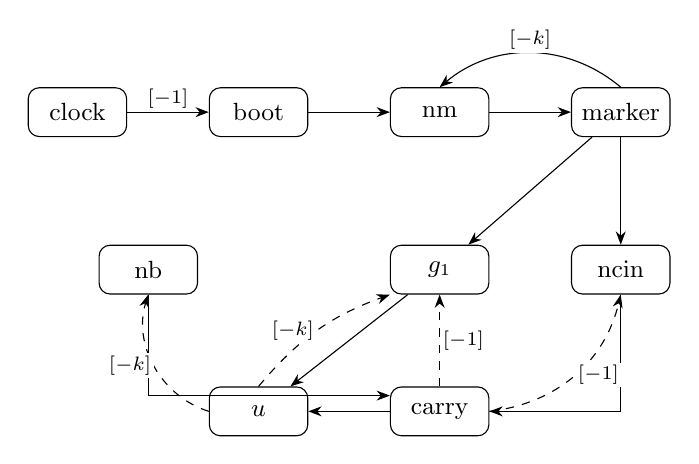
\begin{tikzpicture}[g/.style={draw,rounded corners,minimum width=1.25cm,minimum height=0.62cm,font=\small,fill=white},
  >=Stealth, lab/.style={font=\scriptsize,fill=white,inner sep=1pt}]
\node[g] (clk) at (0,0) {clock};
\node[g] (boot) at (2.3,0) {boot};
\node[g] (nm) at (4.6,0) {nm};
\node[g] (mk) at (6.9,0) {marker};
\node[g] (nb) at (0.9,-2) {nb};
\node[g] (g1) at (4.6,-2) {$g_1$};
\node[g] (ncin) at (6.9,-2) {ncin};
\node[g] (carry) at (4.6,-3.8) {carry};
\node[g] (u) at (2.3,-3.8) {$u$};
\draw[->] (clk) -- node[lab,above]{$[-1]$} (boot);
\draw[->] (boot) -- (nm);
\draw[->] (nm) -- (mk);
\draw[->] (mk.north) to[bend right=40] node[lab,above]{$[-k]$} (nm.north);
\draw[->] (mk) -- (ncin);
\draw[->] (mk) -- (g1);
\draw[->] (ncin) |- (carry);
\draw[->] (nb) |- ([yshift=2mm]carry.west);
\draw[->] (g1) -- (u);
\draw[->] (carry) -- (u);
\draw[->,dashed] (carry.east) to[bend right=35] node[lab,right]{$[-1]$} (ncin.south);
\draw[->,dashed] (carry.north) -- node[lab,right]{$[-1]$} (g1.south);
\draw[->,dashed] (u.west) to[bend left=45] node[lab,left]{$[-k]$} (nb.south);
\draw[->,dashed] (u.north) to[bend left=15] node[lab,left]{$[-k]$} (g1.south west);
\end{tikzpicture}
\caption{The NOR circuit of the bit-serial counter.  Solid edges have delay $0$ (same block);
dashed edges read an earlier block ($[-1]$: previous block, $[-k]$: the same bit of the previous
word).}
\label{fig:circuit}
\end{figure}

\begin{lemma}\label{lem:closed}
Let $\low(w,i)=[\,w\bmod 2^i=2^i-1\,]$ (the lowest $i$ bits of $w$ are all $1$) and let
$\mathrm{bit}_i(x)$ denote bit $i$ of $x$.  The unique solution of the NOR equations is
\begin{align*}
\mathrm{boot}(\tau)&=[\tau=0], & \mathrm{marker}(\tau)&=[k\mid\tau], & \mathrm{nm}&=\neg\mathrm{marker},\\
\mathrm{ncin}(\tau)&=\neg\low(w,i), & \mathrm{nb}(\tau)&=\neg\mathrm{bit}_i(w), &
g_1(\tau)&=\neg(\mathrm{bit}_i(w)\vee\low(w,i)),\\
\mathrm{carry}(\tau)&=\low(w,i+1), & u(\tau)&=\mathrm{bit}_i(w+1).
\end{align*}
In words: word $w$ (blocks $wk,\dots,wk+k-1$) holds the number $(w+1)\bmod 2^k$ in binary, least
significant bit first.
\end{lemma}

\begin{proof}
Each equation is checked directly.  The two arithmetic facts needed are the carry rule
$\low(w,i+1)=\mathrm{bit}_i(w)\wedge\low(w,i)$ and the increment rule
$\mathrm{bit}_i(w+1)=\mathrm{bit}_i(w)\oplus\low(w,i)$; for $u[-k]$ one uses that block $\tau-k$
belongs to word $w-1$, whose value is $w$.  The carry into bit $i$ is
$\mathrm{carry}[-1]\vee\mathrm{marker}=\low(w,i)$.  Uniqueness is immediate by induction on $\tau$.
\end{proof}

\section{The concrete design}

A design implementing the counter with $B=377$, $17$ clocks and $54$ taps was found by computer
search (Section~\ref{sec:search}):
\begin{center}\small
\begin{tabular}{ll}
\toprule
clocks $C$ & $1,4,37,61,100,125,126,152,163,188,189,245,251,262,276,294,338$\\
wires $\rho$ & boot $0$, nm $5$, marker $18$, ncin $38$, nb $64$, $g_1$ $101$, carry $149$, $u$ $219$\\
\bottomrule
\end{tabular}
\end{center}
With $K=k-1$ the move set is $S_k=\{(aK+b)\cdot 377+\delta\}$ over the $54$ taps; for example
\begin{multline*}
S_3=\{2,5,7,8,9,10,12,13,15,16,20,21,22,28,29,35,41,42,47,50,53,55,58,\\
66,69,70,71,79,80,81,83,85,86,90,98,111,118,123,156,177,180,203,\\
221,248,266,309,329,332,335,370,375,976,1013,1118\}.
\end{multline*}
Only three taps depend on $k$ (the long delays feeding nm, nb and $g_1$); the other $51$ moves are
fixed.  Conditions \ref{c:K}--\ref{c:Z0} are finite and are verified mechanically.
Figure~\ref{fig:bitmap} shows the resulting P-positions for $k=3$.

\begin{figure}[t]
\centering
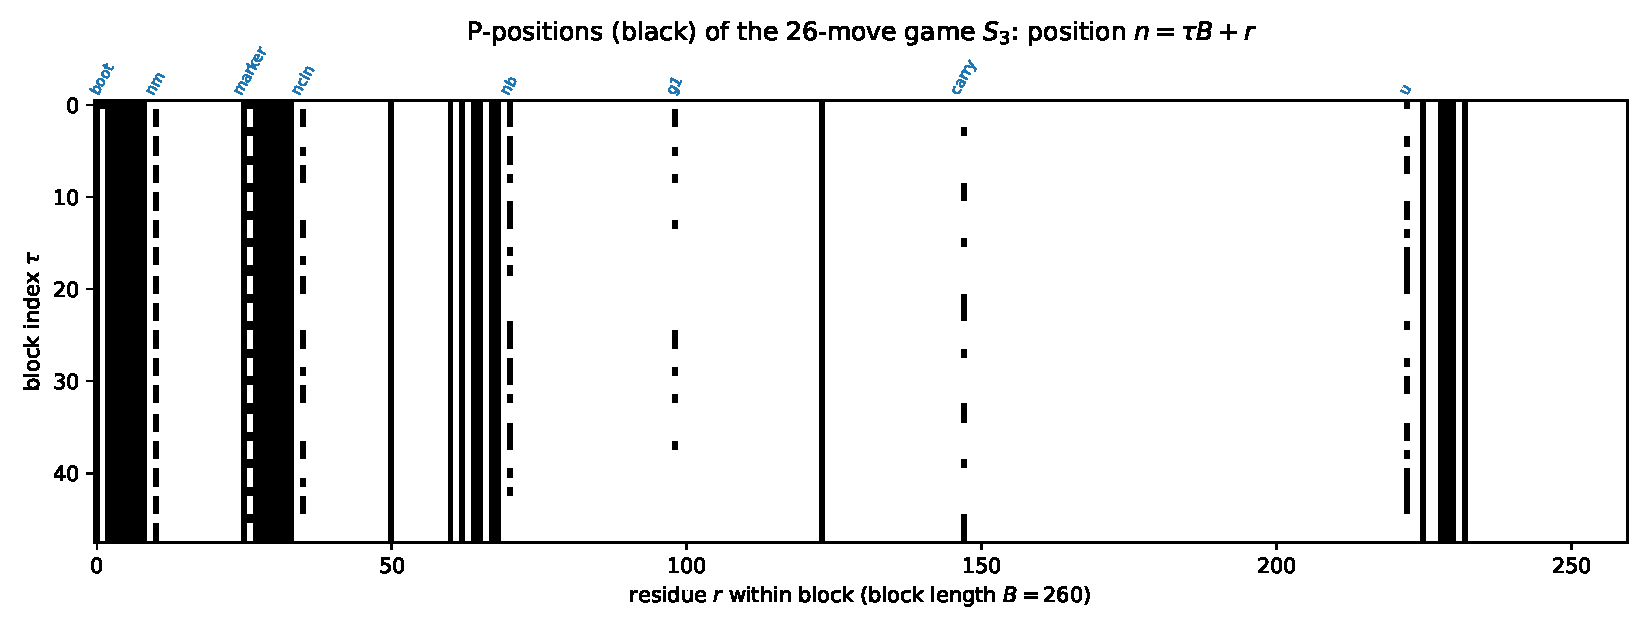
\includegraphics[width=\textwidth]{figs/bitmap.pdf}\\[2mm]
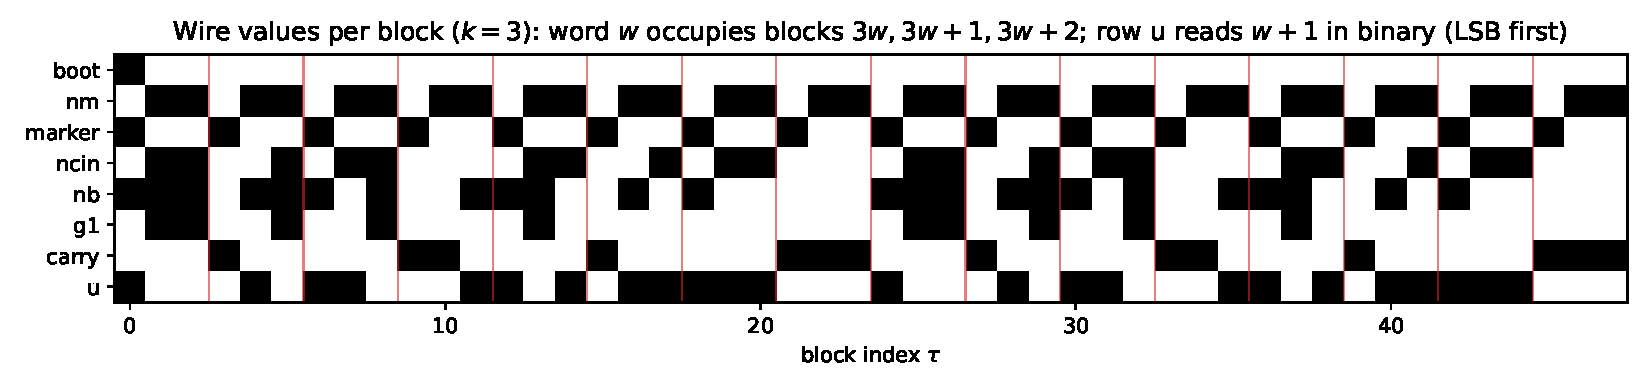
\includegraphics[width=\textwidth]{figs/wires.pdf}
\caption{Top: P-positions of the $54$-move game $S_3$, one block of $377$ positions per row.  Clocks
are the solid columns; the dashed columns are the eight wires.  Bottom: the wire values; the $u$ row
spells $1,2,3,\dots,7,0,1,\dots$ in binary, three blocks per word.  The period is
$377\cdot 3\cdot 2^3=9048$.}
\label{fig:bitmap}
\end{figure}

\section{The least period}

\begin{theorem}\label{thm:period}
For $k\ge2$ the outcome sequence of $S_k$ satisfies $w(n+P)=w(n)$ for all $n\ge B$, where
$P=B\,k\,2^k$, and every eventual period of $w$ is a multiple of $P$.
\end{theorem}

\begin{proof}
Periodicity follows from Theorem~\ref{thm:sim} and Lemma~\ref{lem:closed}: all closed forms depend
only on $\tau\bmod k$ and $(\tau\div k)\bmod 2^k$ except $\mathrm{boot}$, which is constant for
$\tau\ge1$.  Conversely let $p$ be an eventual period.
(1) If $B\nmid p$, then (a finite check) some clock $c$ is shifted by $p\bmod B$ onto a zero residue,
so $w(\tau B+c)=1\neq 0=w(\tau B+c+p)$ for large $\tau$; hence $p=Bm$.
(2) The marker wire gives $[k\mid \tau+m]=[k\mid\tau]$ for all large $\tau$, hence $k\mid m$, say
$m=km'$.
(3) The $u$ wire gives $\mathrm{bit}_i(w+m'+1)=\mathrm{bit}_i(w+1)$ for all $i<k$ and large $w$,
hence $2^k\mid m'$.  Thus $P\mid p$.
\end{proof}

Theorem~\ref{thm:main} follows, and Corollary~\ref{cor:guy} follows because $2^k$ eventually
exceeds $C(377(k+1))^d$.

\section{How the design was found}\label{sec:search}

\begin{enumerate}[leftmargin=*]
\item \textbf{Exploration.}  A C program computes outcome periods by cycle detection on the
$m$-bit shift-register state.  Record periods of max-symmetric five-move sets grow roughly like
$2^{0.33m}$ (confirming Flammenkamp), but along every structured one-parameter family we tried the
periods were erratic---chaotic dynamics that resist proof.  This motivated \emph{designing} rather
than \emph{finding} long periods.
\item \textbf{Layouts.}  Random layouts almost never work: small differences between residues
collide.  Placing wires on a coarse grid $G\cdot Y$ with $Y$ a Sidon set, and clocks in a few
residue classes modulo $G$ chosen so that their sums and differences avoid each other, produced the
first valid design ($B=1157$, $1061$ moves), confirmed by direct simulation for $k\le 8$.
\item \textbf{Optimisation.}  Choosing covering taps by greedy set cover (one tap can cover a zero
residue for many clocks at once) and then running simulated annealing over wire positions, clock
sets and $B$ reduced the number of moves $1061\to169\to 67\to 56\to 54$ (and $53$ with $B=393$).
Every candidate was checked by an exact verifier of conditions \ref{c:K}--\ref{c:Z0} and the final
designs by simulating the game itself.
\end{enumerate}

\section{Formal verification in Lean}\label{sec:lean}

The development (about 1700 lines, Lean 4.33.1, Mathlib) consists of:
\begin{center}\small
\begin{tabular}{ll}
\toprule
\texttt{Basic.lean} & P-set characterisation, uniqueness, computable \texttt{outcome}\\
\texttt{Arith.lean} & block arithmetic (Lemma~\ref{lem:arith})\\
\texttt{Simulation.lean} & designs, conditions \ref{c:K}--\ref{c:Z0}, Theorem~\ref{thm:sim}\\
\texttt{Bits.lean}, \texttt{Counter.lean} & carry/increment rules, Lemma~\ref{lem:closed}\\
\texttt{Design.lean} & the concrete design; all finite conditions by \texttt{decide +kernel}\\
\texttt{Period.lean} & Theorem~\ref{thm:period}\\
\texttt{Main.lean}, \texttt{Grundy.lean} & Theorem~\ref{thm:main}, Corollary~\ref{cor:guy}, nim-values\\
\texttt{Tests.lean} & sanity checks ($\{1,2\}$, $\{1,3,4\}$), Corollary~\ref{cor:guy} with $\max S$\\
\texttt{Layout.lean} & General Layout Lemma (Lemma~\ref{lem:gll}), \texttt{GLL.simulate}\\
\bottomrule
\end{tabular}
\end{center}
The game semantics are defined independently of the construction: \texttt{outcome L n} is defined by
well-founded recursion as ``no legal move leads to a position with \texttt{outcome = true}'', and
\texttt{grundy L n} as the minimum excludant of the options' values.  No \texttt{sorry},
\texttt{native\_decide} or additional axioms are used.

\section{Universality and PSPACE-completeness}\label{sec:pspace}

The counter was laid out by computer search, but a layout exists for \emph{every} NOR circuit.

\begin{definition}[Circuit]\label{def:circuit}
A \emph{circuit} has wires $0,1,\dots,W-1$; every wire $j$ has a finite list $\mathrm{In}(j)$ of inputs
$(\sigma,d)$, where $\sigma$ is a wire or \textsc{clk} and $d=aK+b$ is a delay.  We require:
(i) $\mathrm{In}(0)=\{(\textsc{clk},1)\}$ (wire $0$ is \emph{boot});
(ii) inputs with delay $0$ come from wires of smaller index;
(iii) no wire is its own input;
(iv) if $\sigma>j$ then $b\ge1$.
\end{definition}

Condition (iii) is necessary: a move that is a multiple of $B$ makes \emph{every} residue read
itself, in particular every clock.

\begin{lemma}[General Layout Lemma]\label{lem:gll}
Let $Y=\{0=y_0<y_1<\dots<y_{W-1}\}$ be a Sidon set (all differences $y_i-y_j$, $i\ne j$, distinct)
with $y_1\ge 2$, let $B'\ge 3y_{W-1}+3$ and $B=13B'$.  Place wire $j$ at residue $13y_j$ and clocks at
$C=\{1,5,12\}$; realise every input $(\sigma,d)$ of wire $j$ by the move $dB+13y_j-\rho(\sigma)$
(where $\rho(\textsc{clk})=5$; for backward edges this is $(d-1)B+(B+13y_j-\rho(\sigma))$), and cover
the zero residues by the rule of Table~\ref{tab:cover}.  Then conditions \ref{c:K}--\ref{c:Z0} hold for
every circuit, so by Theorem~\ref{thm:sim} the subtraction game simulates the circuit.  The design has
$B=O(W^2)$ and at most $B+2+\sum_j|\mathrm{In}(j)|$ moves.
\end{lemma}

\begin{table}[t]
\centering\small
\begin{tabular}{ll}
\toprule
residue $r=13z+\rho$, $z\ge1$ & covering clock $c$ (move $r-c$)\\
\midrule
$\rho\in\{0,1,2,9\}$ & $c=5$\\
$\rho\in\{4,5,8,11,12\}$ & $c=1$\\
$\rho\in\{3,7,10\}$ & $c=1$, except $c=5,12,12$ respectively when $z=B'-1$\\
$\rho=6$ & $c=12$, except $c=1$ when $z=1$\\
\midrule
residue $r<13$ & moves\\
\midrule
$r=3,4$ & $r-1$ \qquad $r=7,8,11$: $r-5$ \qquad $r=9,10$: $r-1$\\
$r=2$ & $B-3$ (clock $5$ of the previous block) and $2$ (boot, block $0$)\\
$r=6$ & $B-6$ (clock $12$ of the previous block) and $6$ (boot, block $0$)\\
\bottomrule
\end{tabular}
\caption{Covering the zero residues in the General Layout Lemma.}
\label{tab:cover}
\end{table}

\begin{proof}
Write residues as $13z+\rho$ with \emph{class} $\rho\in[0,13)$ and \emph{coarse index} $z\in[0,B')$.
Let $X$ be the set of wire and clock residues.  A direct computation gives the classes of the
differences $X-X \pmod B$, as coarse sets modulo $B'$:
\[
\begin{array}{c|ccccccccc}
\text{class} & 0 & 1 & 5 & 8 & 12 & 4,7,11 & 2,6,9 & 3,10\\\hline
\text{coarse} & Y-Y & (Y-1)\cup(-Y) & -Y & Y-1 & (Y-1)\cup(-Y) & \{0\} & \{-1\} & \emptyset
\end{array}
\]
(for instance class $8$ consists of $13y-5$, wire minus clock $5$, with coarse index $y-1$).
Since $Y\subset[0,B'/3)$, these coarse sets do not wrap around.

\emph{Intended moves.}  A wire--wire move has residue $13(y_j-y_i)$.  Applied at a clock it lands in
the clock's class with nonzero coarse index, i.e.\ on a zero residue.  Applied at wire $m$ it lands on
a wire only if $y_m-y_j+y_i\in Y$; as $Y\subset[0,B'/3)$ this is an equality of integers
$y_m+y_i=y_j+y_l$, so the Sidon property forces $m=j$ (the intended target), because $i\ne j$ by
(iii).  A clock move has residue $13y_j-5$ (class $8$); applied at wire $m$ it lands in class $5$ with
coarse index $y_m-y_j$, a clock only if $m=j$; applied at a clock $c$ it lands in class
$c+5\in\{6,10,4\}$, which contains no element of $X$.  Hence \ref{c:W} and \ref{c:W2} hold.

\emph{Covering moves.}  For $z\ge1$ every clock lies below $r$, and the move $r-c$ has class
$\rho-c$ (coarse index $z$) or $\rho-c+13$ (coarse index $z-1$).  Reading off the table of $X-X$, the
choices in Table~\ref{tab:cover} are never differences of two elements of $X$: e.g.\ for $\rho=0$,
$c=5$ gives class $8$ with coarse index $z-1$, which is bad only if $z\in Y$, impossible for a zero
residue of class $0$; for $\rho=3$, $c=1$ gives class $2$, bad only if $z=B'-1$, and then $c=5$ gives
class $11$ with coarse index $B'-2\ne0$.  The remaining cases are identical in nature and use only
$1\notin Y$, $B'-1\notin Y$ and $Y\cap(B'-Y)=\emptyset$.  The residues below $13$ are checked
directly.  Since no covering move is a difference of two elements of $X$, covering moves never make a
clock or a wire see anything, which completes \ref{c:K}, and \ref{c:Z1}, \ref{c:Z0} hold by
construction (boot has value $1$ in block $0$).
\end{proof}

Lemma~\ref{lem:gll} is formally verified in Lean (\texttt{Layout.lean}): the proof reduces every
condition to linear arithmetic modulo $13$ with explicit case splits, discharged by \texttt{omega},
plus one application of the Sidon property.  Before formalising it we also checked it
computationally on $1000$ random circuits with up to $40$ wires and random Sidon sets.

\begin{theorem}[PSPACE-completeness]\label{thm:pspace}
The problem
\begin{center}
\textsc{SubGame}: given a finite set $S\subset\N_{>0}$ in unary and $n\in\N$ in binary, is $n$ a
P-position of the subtraction game $S$?
\end{center}
is PSPACE-complete.
\end{theorem}

\begin{proof}
\emph{Membership.}  Compute $w(0),w(1),\dots,w(n)$ keeping only the last $\max S$ values and a
binary counter: space $O(\max S+\log n)$.

\emph{Hardness.}  Fix a deterministic single-tape machine $M$ that decides a PSPACE-complete language
in linear space: on input $x\in\{0,1\}^N$ it works on the tape $\vdash x\dashv$ of length
$L=N+2$, never crosses the end markers, and always halts; modify it so that the accepting state is
absorbing.  Let $T_M(L)\le 2^{cL}$ bound its running time.

\emph{Cellular automaton.}  A cell state is (tape symbol, head state or none, flag).  The usual local
rule simulates one step of $M$; in addition the new flag is the OR of the three old flags and of
``the head is now in the accepting state''.  Encode states in $b=O(1)$ bits so that the all-zero code
(blank, no head, flag $0$) is mapped to itself.

\emph{Bit-serial circuit.}  Block $\tau=tL+i$ carries cell $i$ at time $t$.  Its three neighbours at
time $t-1$ are the blocks $\tau-L-1,\tau-L,\tau-L+1$, i.e.\ delays $K+3,K+2,K+1$ with $K=L-2$.  (At the
seam of the ring the ``neighbours'' are wrong cells, but they are the end markers or cells adjacent
to them, and $M$ never moves the head across a marker; flags are monotone, so reading a flag from a
different time is harmless.)  A fixed NOR circuit computes the rule; each output bit $j$ is OR-ed
with $\mathrm{init}_j=\mathrm{OR}_{i\in I_j}\mathrm{boot}[-i]$, where $I_j$ is the set of cells whose
initial state has bit $j$ equal to $1$.  In the first $L$ blocks all neighbour reads are $0$, so the
rule outputs the zero code and the OR loads the initial configuration.

\emph{Game.}  The circuit has a fixed number $W$ of wires (independent of $x$), so by
Lemma~\ref{lem:gll} it is realised by a design with a \emph{constant} block length $B$.  The move set
$S_x$ has $O(N)$ moves, all at most $(K+4)B=O(N)$, so its unary description has polynomial size, and
it is computable in polynomial time from $x$.  Let $t^*=2^{c'L}\ge T_M(L)+L$ and
$n^*=(t^*L+1)B+13y_{\mathrm{flag}}$.  By Theorem~\ref{thm:sim}, $n^*$ is a P-position of $S_x$ iff the
flag of cell $1$ is set at time $t^*$, iff $M$ accepts $x$.  The binary length of $n^*$ is $O(N)$.
\end{proof}

\begin{theorem}[Binary move sets]\label{thm:exptime}
If the move set $S$ is given in binary (and $n$ in binary), deciding whether $n$ is a P-position of
$S$ is EXPTIME-complete.
\end{theorem}

\begin{proof}
\emph{Membership.}  The simulation above uses space $O(\max S+\log n)$ and time $O(n|S|)$, both at
most exponential in the input length.

\emph{Hardness.}  Repeat the reduction of Theorem~\ref{thm:pspace} for a fixed machine $M$ deciding an
EXPTIME-complete language in time $T(N)=2^{N^c}$, on a tape of length $L=T(N)+2$ (so $M$ never
reaches the right marker).  The circuit and hence $B$ are unchanged.  The three long moves now have
size about $LB$, but in binary they need only $O(N^c)$ bits; the initial configuration is blank
except for the $N$ input cells and the two markers, so only $O(N)$ initialisation moves are needed.
The query position $n^*=(t^*L+1)B+13y_{\mathrm{flag}}$ with $t^*=T(N)+L$ has $O(N^c)$ bits.  Hence
$(S_x,n^*)$ has polynomial size.
\end{proof}

Thus the complexity of one-heap subtraction games is governed by the size of the largest move: they
are easy for every fixed game, PSPACE-complete when the moves are written in unary, and
EXPTIME-complete when they are written in binary.

\begin{corollary}[Periods are hard to compute]\label{cor:perhard}
Given $S$ in unary and $p$ in binary, deciding whether the least outcome period of $S$ exceeds $p$
is PSPACE-hard.
\end{corollary}

\begin{proof}
In the reduction of Theorem~\ref{thm:pspace} make both halting states absorbing; after $M$ halts
the cellular automaton is frozen, so all wires become periodic with period $L$ (blocks).  Add a
$L$-bit serial counter as in Section~\ref{sec:counter} whose carry-in is additionally AND-ed with
the flag of the current cell.  If $M$ rejects, the counter never moves and the eventual period
divides $BL$; if $M$ accepts, the counter eventually runs and, as in Theorem~\ref{thm:period}, the
least period is a multiple of $BL2^L$.  Take $p=BL$.
\end{proof}

\section{Discussion and open problems}

\begin{enumerate}[leftmargin=*]
\item \textbf{How few moves?}  Our construction needs $54$ moves; Flammenkamp's data suggest that
five moves may already give exponential periods.  What is the least $n$ for which periods of
$n$-move games are not polynomially bounded?
\item \textbf{Growth rate.}  Our periods grow like $2^{\max S/377}$, much slower than the empirical
$2^{0.3\max S}$ of Flammenkamp's records.  Can one prove $2^{c\max S}$ for a larger $c$?
\item \textbf{Bounded number of moves.}  Our hardness reductions use $O(N)$ moves.  Is
\textsc{SubGame} still PSPACE-hard (or EXPTIME-hard, in binary) when the number of moves is bounded?
\item \textbf{Periods.}  Theorem~\ref{thm:pspace} suggests that computing the period of a given
subtraction game is PSPACE-hard as well.
\end{enumerate}

\begin{thebibliography}{9}
\bibitem{AB} I.~Althöfer and J.~Bültermann, Superlinear period lengths in some subtraction games,
\emph{Theoret.\ Comput.\ Sci.} 148 (1995) 111--119.
\bibitem{WW} E.~R.~Berlekamp, J.~H.~Conway and R.~K.~Guy, \emph{Winning Ways for Your Mathematical
Plays}, A K Peters, 2001--2004.
\bibitem{Flammenkamp} A.~Flammenkamp, \emph{Lange Perioden in Subtraktions-Spielen}, Dissertation,
Universität Bielefeld, 1997.
\bibitem{LS} U.~Larsson and I.~Saha, A brief conversation about subtraction games,
arXiv:2405.20054 (2024); in \emph{Games of No Chance 6}.
\bibitem{LW} U.~Larsson and J.~Wästlund, From heaps of matches to the limits of computability,
\emph{Electron.\ J.\ Combin.} 20 (2013) P41.
\bibitem{DGPS} K.~Burke, A.~Dailly and N.~Oijid, Complexity and algorithms for Arc-Kayles and
Non-Disconnecting Arc-Kayles, arXiv:2404.10390 (2024).
\bibitem{GV} V.~Gurvich and M.~Vyalyi, On computational hardness of multidimensional subtraction
games, \emph{Algorithms} 14 (2021) 71, arXiv:2001.03962.
\bibitem{L12} U.~Larsson, Impartial games emulating one-dimensional cellular automata and
undecidability, arXiv:1201.1039 (2012).
\bibitem{MP} I.~Miklós and L.~Post, Superpolynomial period lengths of the winning positions in the
subtraction game, \emph{Int.\ J.\ Game Theory} (2024), arXiv:2312.02426.
\bibitem{Nowakowski} R.~J.~Nowakowski, Unsolved problems in combinatorial games, in \emph{Games of
No Chance 5}, MSRI Publ.\ 70 (2019) 125--168.
\bibitem{Ward} M.~D.~Ward, A conjecture about periods in subtraction games, arXiv:1606.04029.
\end{thebibliography}

\end{document}
